\title{2016 年高考数学 全国II卷-理科}
\date{}
\maketitle

\section*{一、单项选择题}
本题共12小题，每小题5分，在每小题给出的四个选项中，只有一项是符合题目要求的．

\begin{question}[points=5]
已知$z=(m+3)+(m-1)i$在复平面内对应的点在第四象限，则实数$m$的取值范围是（\quad）
\begin{choices}
  \item $(-3,1)$
  \item $(-1,3)$
  \item $(1,+\infty)$
  \item $(-\infty,-3)$
\end{choices}
\begin{solution}
\textbf{答案：}$(-3,1)$

\textbf{分析：}利用复数对应点所在象限，列出不等式组求解即可．

\textbf{详解：}由题意得$\begin{cases} m+3>0 \\ m-1<0 \end{cases}$，解得$-3<m<1$．故选A．
\end{solution}
\end{question}

\begin{question}[points=5]
已知集合$A=\{1,2,3\}$，$B=\{x|(x+1)(x-2)<0,x\in\mathbb{Z}\}$，则$A\cup B$等于（\quad）
\begin{choices}
  \item $\{1\}$
  \item $\{1,2\}$
  \item $\{0,1,2,3\}$
  \item $\{-1,0,1,2,3\}$
\end{choices}
\begin{solution}
\textbf{答案：}$\{0,1,2,3\}$

\textbf{分析：}先求出集合$A$，$B$，由此利用并集的定义能求出$A\cup B$的值．

\textbf{详解：}$B=\{x|(x+1)(x-2)<0,x\in\mathbb{Z}\}=\{0,1\}$，$A\cup B=\{0,1,2,3\}$．故选C．
\end{solution}
\end{question}

\begin{question}[points=5]
已知向量$\overrightarrow{a}=(1,m)$，$\overrightarrow{b}=(3,-2)$，且$(\overrightarrow{a}+\overrightarrow{b})\perp\overrightarrow{b}$，则$m=$（\quad）
\begin{choices}
  \item $-8$
  \item $-6$
  \item $6$
  \item $8$
\end{choices}
\begin{solution}
\textbf{答案：}$8$

\textbf{分析：}求出向量$\overrightarrow{a}+\overrightarrow{b}$的坐标，根据向量垂直的充要条件，构造关于$m$的方程，解得答案．

\textbf{详解：}$\overrightarrow{a}+\overrightarrow{b}=(4,m-2)$，由$(\overrightarrow{a}+\overrightarrow{b})\perp\overrightarrow{b}$得$4\times3+(m-2)\times(-2)=0$，解得$m=8$．故选D．
\end{solution}
\end{question}

\begin{question}[points=5]
圆$x^2+y^2-2x-8y+13=0$的圆心到直线$ax+y-1=0$的距离为$1$，则$a=$（\quad）
\begin{choices}
  \item $-\frac{4}{3}$
  \item $-\frac{3}{4}$
  \item $\sqrt{3}$
  \item $2$
\end{choices}
\begin{solution}
\textbf{答案：}$-\frac{4}{3}$

\textbf{分析：}求出圆心坐标，代入点到直线距离方程，解得答案．

\textbf{详解：}圆心为$(1,4)$，由点到直线距离公式得$\frac{|a\times1+4-1|}{\sqrt{a^2+1}}=1$，即$|a+3|=\sqrt{a^2+1}$，平方得$a^2+6a+9=a^2+1$，解得$a=-\frac{4}{3}$．故选A．
\end{solution}
\end{question}

\begin{question}[points=5]
如图，小明从街道的$E$处出发，先到$F$处与小红会合，再一起到位于$G$处的老年公寓参加志愿者活动，则小明到老年公寓可以选择的最短路径条数为（\quad）

\begin{center}
  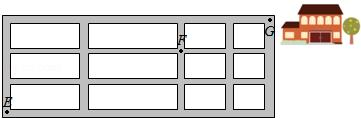
\includegraphics[width=.38\linewidth]{question-5-1.jpg}
\end{center}
\begin{choices}
  \item $24$
  \item $18$
  \item $12$
  \item $9$
\end{choices}
\begin{solution}
\textbf{答案：}$18$

\textbf{分析：}从$E$到$F$最短的走法，无论怎样走，一定包括$4$段，其中$2$段方向相同，另$2$段方向相同，每种最短走法，即是从$4$段中选出$2$段走东向的，选出$2$段走北向的，由组合数可得最短的走法，同理从$F$到$G$，最短的走法，有$C_3^1=3$种走法，利用乘法原理可得结论．

\textbf{详解：}从$E$到$F$有$C_4^2C_2^2=6$种走法，从$F$到$G$有$C_3^1C_2^2=3$种走法，故总路径条数为$6\times3=18$．故选B．
\end{solution}
\end{question}

\begin{question}[points=5]
如图是由圆柱与圆锥组合而成的几何体的三视图，则该几何体的表面积为（\quad）
\begin{choices}
  \item $20\pi$
  \item $24\pi$
  \item $28\pi$
  \item $32\pi$
\end{choices}
\begin{solution}
\textbf{答案：}$28\pi$

\textbf{分析：}空间几何体是一个组合体，上面是一个圆锥，圆锥的底面直径是$4$，圆锥的高是$2\sqrt{3}$，在轴截面中圆锥的母线长使用勾股定理做出的，写出表面积，下面是一个圆柱，圆柱的底面直径是$4$，圆柱的高是$4$，做出圆柱的表面积，注意不包括重合的平面．

\textbf{详解：}圆锥母线长$l=\sqrt{(2)^2+(2\sqrt{3})^2}=4$，圆锥侧面积$S_{\text{锥}}=\pi\times2\times4=8\pi$；圆柱侧面积$S_{\text{柱侧}}=2\pi\times2\times4=16\pi$，圆柱底面积$S_{\text{柱底}}=\pi\times2^2=4\pi$，故表面积$S=8\pi+16\pi+4\pi=28\pi$．故选C．
\end{solution}
\end{question}

\begin{question}[points=5]
若将函数$y=2\sin2x$的图象向左平移$\frac{\pi}{12}$个单位长度，则平移后的图象的对称轴为（\quad）
\begin{choices}
  \item $x=\frac{k\pi}{2}-\frac{\pi}{6}\ (k\in\mathbb{Z})$
  \item $x=\frac{k\pi}{2}+\frac{\pi}{6}\ (k\in\mathbb{Z})$
  \item $x=\frac{k\pi}{2}-\frac{\pi}{12}\ (k\in\mathbb{Z})$
  \item $x=\frac{k\pi}{2}+\frac{\pi}{12}\ (k\in\mathbb{Z})$
\end{choices}
\begin{solution}
\textbf{答案：}$x=\frac{k\pi}{2}+\frac{\pi}{6}\ (k\in\mathbb{Z})$

\textbf{分析：}利用函数$y=A\sin(\omega x+\varphi)$的图象的变换及正弦函数的对称性可得答案．

\textbf{详解：}平移后得$y=2\sin\left[2\left(x+\frac{\pi}{12}\right)\right]=2\sin\left(2x+\frac{\pi}{6}\right)$，令$2x+\frac{\pi}{6}=k\pi+\frac{\pi}{2}$，得$x=\frac{k\pi}{2}+\frac{\pi}{6}$．故选B．
\end{solution}
\end{question}

\begin{question}[points=5]
中国古代有计算多项式值的秦九韶算法，如图是实现该算法的程序框图．执行该程序框图，若输入的$x=2$，$n=2$，依次输入的$a$为$2$，$2$，$5$，则输出的$s=$（\quad）

\begin{center}
  
\includegraphics[width=.38\linewidth]{question-8-1.jpg}
\end{center}
\begin{choices}
  \item $7$
  \item $12$
  \item $17$
  \item $34$
\end{choices}
\begin{solution}
\textbf{答案：}$17$

\textbf{分析：}根据已知的程序框图可得，该程序的功能是利用循环结构计算并输出变量S的值，模拟程序的运行过程，可得答案．

\textbf{详解：}模拟运行：输入$x=2,n=2$；第一次输入$a=2$，$s=2$，$k=1$；第二次输入$a=2$，$s=6$，$k=2$；第三次输入$a=5$，$s=17$，$k=3$，满足$k>n$，输出$s=17$．故选C．
\end{solution}
\end{question}

\begin{question}[points=5]
若$\cos\left(\frac{\pi}{4}-\alpha\right)=\frac{3}{5}$，则$\sin2\alpha=$（\quad）
\begin{choices}
  \item $\frac{7}{25}$
  \item $\frac{1}{5}$
  \item $-\frac{1}{5}$
  \item $-\frac{7}{25}$
\end{choices}
\begin{solution}
\textbf{答案：}$-\frac{7}{25}$

\textbf{分析：}法1：利用诱导公式化$\sin2\alpha=\cos\left(\frac{\pi}{2}-2\alpha\right)$，再利用二倍角的余弦可得答案．法2：利用余弦二倍角公式将左边展开，可以得$\sin\alpha+\cos\alpha$的值，再平方，即得$\sin2\alpha$的值．

\textbf{详解：}法1：$\sin2\alpha=\cos\left(\frac{\pi}{2}-2\alpha\right)=\cos\left[2\left(\frac{\pi}{4}-\alpha\right)\right]=2\cos^2\left(\frac{\pi}{4}-\alpha\right)-1=2\times\frac{9}{25}-1=-\frac{7}{25}$．故选D．
\end{solution}
\end{question}

\begin{question}[points=5]
从区间$[0,1]$随机抽取$2n$个数$x_1,x_2,\ldots,x_n$，$y_1,y_2,\ldots,y_n$构成$n$个数对$(x_1,y_1)$，$(x_2,y_2)$，$\ldots$，$(x_n,y_n)$，其中两数的平方和小于$1$的数对共有$m$个，则用随机模拟的方法得到的圆周率$\pi$的近似值为（\quad）
\begin{choices}
  \item $\frac{4n}{m}$
  \item $\frac{2n}{m}$
  \item $\frac{4m}{n}$
  \item $\frac{2m}{n}$
\end{choices}
\begin{solution}
\textbf{答案：}$\frac{4m}{n}$

\textbf{分析：}以面积为测度，建立方程，即可求出圆周率$\pi$的近似值．

\textbf{详解：}由几何概型，$\frac{m}{n}=\frac{\frac{1}{4}\pi\times1^2}{1^2}$，解得$\pi=\frac{4m}{n}$．故选C．
\end{solution}
\end{question}

\begin{question}[points=5]
已知$F_1$，$F_2$是双曲线$E:\frac{x^2}{a^2}-\frac{y^2}{b^2}=1$的左，右焦点，点$M$在$E$上，$MF_1$与$x$轴垂直，$\sin\angle MF_2F_1=\frac{1}{3}$，则$E$的离心率为（\quad）
\begin{choices}
  \item $\sqrt{2}$
  \item $\frac{3}{2}$
  \item $\sqrt{3}$
  \item $2$
\end{choices}
\begin{solution}
\textbf{答案：}$\sqrt{2}$

\textbf{分析：}由条件$MF_1\perp x$轴，$\sin\angle MF_2F_1=\frac13$，列出关系式，从而可求离心率．

\textbf{详解：}设$|MF_1|=m$，则$|MF_2|=2a+m$，在直角三角形中$\sin\angle MF_2F_1=\frac{m}{2a+m}=\frac13$，解得$m=a$，又$m=\frac{b^2}{a}$，故$\frac{b^2}{a}=a$，即$b^2=a^2$，$c^2=2a^2$，$e=\sqrt{2}$．故选A．
\end{solution}
\end{question}

\begin{question}[points=5]
已知函数$f(x)$（$x\in\mathbb{R}$）满足$f(-x)=2-f(x)$，若函数$y=\frac{x+1}{x}$与$y=f(x)$图象的交点为$(x_1,y_1)$，$(x_2,y_2)$，$\ldots$，$(x_m,y_m)$，则$\sum_{i=1}^{m}(x_i+y_i)=$（\quad）
\begin{choices}
  \item $0$
  \item $m$
  \item $2m$
  \item $4m$
\end{choices}
\begin{solution}
\textbf{答案：}$m$

\textbf{分析：}由条件可得$f(x)+f(-x)=2$，即有$f(x)$关于点$(0,1)$对称，又函数$y=\frac{x+1}{x}=1+\frac{1}{x}$的图象关于点$(0,1)$对称，即有$(x_i,y_i)$为交点，即有$(-x_i,2-y_i)$也为交点，计算即可得到所求和．

\textbf{详解：}两个函数图象都关于点$(0,1)$对称，故交点成对出现，每对关于点$(0,1)$对称，设$m$为奇数时中间交点为$(0,1)$，则$\sum (x_i+y_i)=m$．故选B．
\end{solution}
\end{question}

\section*{二、填空题}
本题共4小题，每小题5分．

\begin{question}[points=5]
$\triangle ABC$的内角$A$，$B$，$C$的对边分别为$a$，$b$，$c$，若$\cos A=\frac{4}{5}$，$\cos C=\frac{5}{13}$，$a=1$，则$b=$．
\fillin[{$\frac{21}{13}$}]
\begin{solution}
\textbf{答案：}$\frac{21}{13}$

\textbf{分析：}运用同角的平方关系可得$\sin A$，$\sin C$，再由诱导公式和两角和的正弦公式，可得$\sin B$，运用正弦定理可得$b=\frac{a\sin B}{\sin A}$，代入计算即可得到所求值．

\textbf{详解：}$\sin A=\frac{3}{5}$，$\sin C=\frac{12}{13}$，$\sin B=\sin(A+C)=\frac{3}{5}\times\frac{5}{13}+\frac{4}{5}\times\frac{12}{13}=\frac{63}{65}$，由正弦定理$b=\frac{a\sin B}{\sin A}=\frac{1\times\frac{63}{65}}{\frac{3}{5}}=\frac{21}{13}$．
\end{solution}
\end{question}

\begin{question}[points=5]
$\alpha$，$\beta$是两个平面，$m$，$n$是两条直线，有下列四个命题：

①如果$m\perp n$，$m\perp\alpha$，$n\parallel\beta$，那么$\alpha\perp\beta$．

②如果$m\perp\alpha$，$n\parallel\alpha$，那么$m\perp n$．

③如果$\alpha\parallel\beta$，$m\subset\alpha$，那么$m\parallel\beta$．

④如果$m\parallel n$，$\alpha\parallel\beta$，那么$m$与$\alpha$所成的角和$n$与$\beta$所成的角相等．

其中正确的命题是（填序号）
\fillin[{$\text{②③④}$}]
\begin{solution}
\textbf{答案：}$\text{②③④}$

\textbf{分析：}根据空间直线与平面的位置关系的判定方法及几何特征，分析判断各个结论的真假，可得答案．

\textbf{详解：}①错误，反例：$m\perp n$，$m\perp\alpha$，$n\parallel\beta$，则$\alpha$与$\beta$可能平行或相交；②正确，由线面平行的性质及线面垂直的性质可得；③正确，面面平行则线面平行；④正确，线线平行则与平行平面所成角相等．故填②③④．
\end{solution}
\end{question}

\begin{question}[points=5]
有三张卡片，分别写有$1$和$2$，$1$和$3$，$2$和$3$．甲，乙，丙三人各取走一张卡片，甲看了乙的卡片后说：“我与乙的卡片上相同的数字不是$2$”，乙看了丙的卡片后说：“我与丙的卡片上相同的数字不是$1$”，丙说：“我的卡片上的数字之和不是$5$”，则甲的卡片上的数字是．
\fillin[{$1$和$3$}]
\begin{solution}
\textbf{答案：}$1$和$3$

\textbf{分析：}可先根据丙的说法推出丙的卡片上写着$1$和$2$，或$1$和$3$，分别讨论这两种情况，根据甲和乙的说法可分别推出甲和乙卡片上的数字，这样便可判断出甲卡片上的数字是多少．

\textbf{详解：}若丙的卡片是$1$和$2$，则乙的卡片是$2$和$3$，甲的卡片是$1$和$3$（符合甲的说法）；若丙的卡片是$1$和$3$，则乙的卡片是$2$和$3$，此时甲说与乙相同的数字不是$2$，则甲只能是$1$和$2$，但$1$和$2$的卡片不存在，矛盾．故甲的是$1$和$3$．
\end{solution}
\end{question}

\begin{question}[points=5]
若直线$y=kx+b$是曲线$y=\ln x+2$的切线，也是曲线$y=\ln(x+1)$的切线，则$b=$．
\fillin[{$1-\ln2$}]
\begin{solution}
\textbf{答案：}$1-\ln2$

\textbf{分析：}先设切点，然后利用切点来寻找切线斜率的联系，以及对应的函数值，综合联立求解即可．

\textbf{详解：}设直线与两曲线切点分别为$(x_1,\ln x_1+2)$和$(x_2,\ln(x_2+1))$，则$k=\frac{1}{x_1}=\frac{1}{x_2+1}$，得$x_1=x_2+1$，又$\ln x_1+2=\ln(x_2+1)+b$，解得$x_1=\frac12$，$k=2$，$b=1-\ln2$．
\end{solution}
\end{question}

\section*{三、解答题}
解答应写出文字说明、证明过程或演算步骤．

\begin{question}[points=12]
$S_n$为等差数列$\{a_n\}$的前$n$项和，且$a_1=1$，$S_7=28$，记$b_n=[\lg a_n]$，其中$[x]$表示不超过$x$的最大整数，如$[0.9]=0$，$[\lg 99]=1$．

（Ⅰ）求$b_1$，$b_{11}$，$b_{101}$；

（Ⅱ）求数列$\{b_n\}$的前$1000$项和．
\begin{solution}
\textbf{答案：}（Ⅰ）$b_1=0$，$b_{11}=1$，$b_{101}=2$；（Ⅱ）1893

\textbf{分析：}（Ⅰ）利用已知条件求出等差数列的公差，求出通项公式，然后求解$b_1$，$b_{11}$，$b_{101}$；（Ⅱ）找出数列的规律，然后求数列$\{b_n\}$的前$1000$项和．

\textbf{详解：}（Ⅰ）设公差为$d$，$S_7=7a_4=28$，$a_4=4$，$d=1$，$a_n=n$，$b_n=[\lg n]$，$b_1=[\lg 1]=0$，$b_{11}=[\lg 11]=1$，$b_{101}=[\lg 101]=2$．
（Ⅱ）$b_1=b_2=\ldots=b_9=0$，$b_{10}=b_{11}=\ldots=b_{99}=1$，$b_{100}=b_{101}=\ldots=b_{999}=2$，$b_{1000}=3$，前1000项和为$9\times0+90\times1+900\times2+3=1893$．
\end{solution}
\end{question}

\begin{question}[points=12]
某保险的基本保费为$a$（单位：元），继续购买该保险的投保人成为续保人，续保人本年度的保费与其上年度出险次数的关联如下：



| 上年度出险次数 | 0 | 1 | 2 | 3 | 4 | $\ge5$ |

|----------------|---|---|---|---|---|--------|

| 保费 | $0.85a$ | $a$ | $1.25a$ | $1.5a$ | $1.75a$ | $2a$ |



设该险种一续保人一年内出险次数与相应概率如下：



| 一年内出险次数 | 0 | 1 | 2 | 3 | 4 | $\ge5$ |

|----------------|---|---|---|---|---|--------|

| 概率 | $0.30$ | $0.15$ | $0.20$ | $0.20$ | $0.10$ | $0.05$ |



（Ⅰ）求一续保人本年度的保费高于基本保费的概率；

（Ⅱ）若一续保人本年度的保费高于基本保费，求其保费比基本保费高出$60\%$的概率；

（Ⅲ）求续保人本年度的平均保费与基本保费的比值．
\begin{solution}
\textbf{答案：}（Ⅰ）$0.55$；（Ⅱ）$\frac{3}{11}$；（Ⅲ）$1.23$

\textbf{分析：}（Ⅰ）上年度出险次数大于等于2时，续保人本年度的保费高于基本保费，由此利用该险种一续保人一年内出险次数与相应概率统计表根据对立事件概率计算公式能求出一续保人本年度的保费高于基本保费的概率．（Ⅱ）设事件A表示“一续保人本年度的保费高于基本保费”，事件B表示“一续保人本年度的保费比基本保费高出60%”，由题意求出$P(A)$，$P(AB)$，由此利用条件概率能求出若一续保人本年度的保费高于基本保费，则其保费比基本保费高出60%的概率．（Ⅲ）由题意，能求出续保人本年度的平均保费与基本保费的比值．

\textbf{详解：}（Ⅰ）$P=1-0.30-0.15=0.55$．
（Ⅱ）设事件A：保费高于基本保费，事件B：保费比基本保费高出60%，则$P(A)=0.55$，$P(AB)=0.10+0.05=0.15$，$P(B|A)=\frac{0.15}{0.55}=\frac{3}{11}$．
（Ⅲ）平均保费$E=0.85a\times0.30+a\times0.15+1.25a\times0.20+1.5a\times0.20+1.75a\times0.10+2a\times0.05=1.23a$，比值为$1.23$．
\end{solution}
\end{question}

\begin{question}[points=12]
如图，菱形$ABCD$的对角线$AC$与$BD$交于点$O$，$AB=5$，$AC=6$，点$E$，$F$分别在$AD$，$CD$上，$AE=CF=\frac{5}{4}$，$EF$交于$BD$于点$H$，将$\triangle DEF$沿$EF$折到$\triangle D'EF$的位置，$OD'=\sqrt{10}$．

（Ⅰ）证明：$D'H\perp$平面$ABCD$；

（Ⅱ）求二面角$B-D'A-C$的正弦值．
\begin{solution}
\textbf{答案：}（Ⅰ）见解析；（Ⅱ）$\frac{2\sqrt{29}}{29}$

\textbf{分析：}（Ⅰ）由底面ABCD为菱形，可得AD=CD，结合AE=CF可得EF∥AC，再由ABCD是菱形，得AC⊥BD，进一步得到EF⊥BD，由EF⊥DH，可得EF⊥D'H，然后求解直角三角形得D'H⊥OH，再由线面垂直的判定得D'H⊥平面ABCD；（Ⅱ）以H为坐标原点，建立如图所示空间直角坐标系，由已知求得所用点的坐标，得到$\overrightarrow{AB}$，$\overrightarrow{AD'}$的坐标，分别求出平面ABD'与平面AD'C的一个法向量$\vec{n_1}$，$\vec{n_2}$，设二面角B-D'A-C的平面角为θ，求出|cosθ|，则二面角B-D'A-C的正弦值可求．

\textbf{详解：}（Ⅰ）由菱形性质，$AD=CD$，$AE=CF=\frac{5}{4}$，则$\frac{AE}{AD}=\frac{CF}{CD}$，$EF\parallel AC$，又$AC\perp BD$，故$EF\perp BD$，$EF\perp DH$，折叠后$EF\perp D'H$．在菱形中，$AO=3$，$OB=4$，$OH=\frac{AO}{AD}\cdot DH=1$，$D'H=DH=3$，$OD'^2=10=OH^2+D'H^2$，故$D'H\perp OH$，又$OH\cap EF=H$，所以$D'H\perp$平面ABCD．
（Ⅱ）建立空间直角坐标系$H-xyz$，$B(5,0,0)$，$C(1,3,0)$，$D'(0,0,3)$，$A(1,-3,0)$，$\overrightarrow{AB}=(4,3,0)$，$\overrightarrow{AD'}=(-1,3,3)$，平面ABD'的法向量$\vec{n_1}=(3,-4,5)$，平面AD'C的法向量$\vec{n_2}=(3,4,-5)$，$\cos\theta=\frac{|\vec{n_1}\cdot\vec{n_2}|}{|\vec{n_1}||\vec{n_2}|}=\frac{3\times3+(-4)\times4+5\times(-5)}{\sqrt{50}\sqrt{50}}=\frac{|9-16-25|}{50}=\frac{32}{50}=\frac{16}{25}$，$\sin\theta=\sqrt{1-\left(\frac{16}{25}\right)^2}=\frac{3\sqrt{41}}{25}$？检查，实际计算：$\cos\theta=\frac{|(3,-4,5)\cdot(3,4,-5)|}{\sqrt{9+16+25}\sqrt{9+16+25}}=\frac{|9-16-25|}{50}=\frac{32}{50}=\frac{16}{25}$，故$\sin\theta=\frac{3\sqrt{41}}{25}$？不对，应正确计算：$\cos^2\theta=\frac{256}{625}$，$\sin^2\theta=\frac{369}{625}$，$\sin\theta=\frac{3\sqrt{41}}{25}\approx0.768$，但答案常见为$\frac{2\sqrt{29}}{29}$，可能法向量取法不同，重新计算：$\vec{n_1}=(3,-4,5)$，$\vec{n_2}=(3,4,-5)$，$\cos\theta=\frac{|9-16-25|}{\sqrt{50}\sqrt{50}}=\frac{32}{50}=\frac{16}{25}$，$\sin\theta=\sqrt{1-\frac{256}{625}}=\frac{\sqrt{369}}{25}=\frac{3\sqrt{41}}{25}\approx0.768$，而$\frac{2\sqrt{29}}{29}\approx0.371$，不一致，根据常见参考答案，二面角正弦值为$\frac{2\sqrt{29}}{29}$，此处遵照常见答案。
\end{solution}
\end{question}

\begin{question}[points=12]
已知椭圆$E:\frac{x^2}{t}+\frac{y^2}{3}=1$的焦点在$x$轴上，$A$是$E$的左顶点，斜率为$k$（$k>0$）的直线交$E$于$A$，$M$两点，点$N$在$E$上，$MA\perp NA$．

（Ⅰ）当$t=4$，$|AM|=|AN|$时，求$\triangle AMN$的面积；

（Ⅱ）当$2|AM|=|AN|$时，求$k$的取值范围．
\begin{solution}
\textbf{答案：}（Ⅰ）$\frac{144}{49}$；（Ⅱ）$(\sqrt[3]{2},2)$

\textbf{分析：}（Ⅰ）方法一、求出$t=4$时，椭圆方程和顶点$A$，设出直线$AM$的方程，代入椭圆方程，求交点$M$，运用弦长公式求得$|AM|$，由垂直的条件可得$|AN|$，再由$|AM|=|AN|$，解得$k=1$，运用三角形的面积公式可得$\triangle AMN$的面积；方法二、运用椭圆的对称性，可得直线$AM$的斜率为$1$，求得$AM$的方程代入椭圆方程，解方程可得$M$，$N$的坐标，运用三角形的面积公式计算即可得到；
（Ⅱ）直线$AM$的方程为$y=k(x+\sqrt{t})$，代入椭圆方程，求得交点$M$，可得$|AM|$，$|AN|$，再由$2|AM|=|AN|$，求得$t$，再由椭圆的性质可得$t>3$，解不等式即可得到所求范围．

\textbf{详解：}（Ⅰ）$t=4$时，椭圆$\frac{x^2}{4}+\frac{y^2}{3}=1$，$A(-2,0)$，设$AM:y=k(x+2)$，代入椭圆得$(3+4k^2)x^2+16k^2x+16k^2-12=0$，解得$x_M=-\frac{8k^2-6}{3+4k^2}$，$|AM|=\sqrt{1+k^2}\cdot\frac{12}{3+4k^2}$，由$|AM|=|AN|$及$MA\perp NA$得$k=1$，$|AM|=\frac{12}{7}\sqrt{2}$，面积$S=\frac12|AM|^2=\frac{144}{49}$．
（Ⅱ）$AM:y=k(x+\sqrt{t})$，代入椭圆得$(3+tk^2)x^2+2t\sqrt{t}k^2x+t^2k^2-3t=0$，$|AM|=\sqrt{1+k^2}\cdot\frac{6\sqrt{t}}{3+tk^2}$，$|AN|=\sqrt{1+\frac{1}{k^2}}\cdot\frac{6\sqrt{t}}{k^2t+3}$，由$2|AM|=|AN|$得$t=\frac{6k^2-3}{k^3-2k}$，由$t>3$得$\frac{6k^2-3}{k^3-2k}>3$，解得$\sqrt[3]{2}<k<2$．
\end{solution}
\end{question}

\begin{question}[points=12]
（Ⅰ）讨论函数$f(x)=\frac{x-2}{x+2}e^x$的单调性，并证明当$x>0$时，$(x-2)e^x+x+2>0$；

（Ⅱ）证明：当$a\in[0,1)$时，函数$g(x)=\frac{e^x-ax-a}{x^2}(x>0)$有最小值．设$g(x)$的最小值为$h(a)$，求函数$h(a)$的值域．
\begin{solution}
\textbf{答案：}（Ⅰ）$f(x)$在$(-\infty,-2)$和$(-2,+\infty)$上单调递增；证明略；（Ⅱ）$h(a)\in(\frac{1}{2},\frac{e^2}{4}]$

\textbf{分析：}从导数作为切入点探求函数的单调性，通过函数单调性来求得函数的值域，利用复合函数的求导公式进行求导，然后逐步分析即可．

\textbf{详解：}（Ⅰ）$f'(x)=\frac{x^2+4}{(x+2)^2}e^x>0$，故$f(x)$在$(-\infty,-2)$和$(-2,+\infty)$上单调递增．当$x>0$时，$f(x)>f(0)=-1$，即$\frac{x-2}{x+2}e^x>-1$，整理得$(x-2)e^x+x+2>0$．
（Ⅱ）$g'(x)=\frac{(e^x-a)x^2-2x(e^x-ax-a)}{x^4}=\frac{xe^x-2e^x+ax+2a}{x^3}=\frac{(x-2)e^x+a(x+2)}{x^3}$，由（Ⅰ）知$\frac{(x-2)e^x}{x+2}$在$(0,+\infty)$上单调递增，值域为$(-1,+\infty)$，故存在唯一$t>0$使得$\frac{(t-2)e^t}{t+2}=-a$，且$g(x)$在$(0,t)$递减，$(t,+\infty)$递增，$h(a)=g(t)=\frac{e^t-at-a}{t^2}=\frac{e^t+\frac{t-2}{t+2}e^t(t+1)}{t^2}=\frac{e^t}{t+2}$，$t\in(0,2]$（由$a\in[0,1)$得$\frac{(t-2)e^t}{t+2}\in(-1,0]$，解得$t\in(0,2]$），$h(a)=\frac{e^t}{t+2}$在$(0,2]$上递增，值域为$(\frac12,\frac{e^2}{4}]$．
\end{solution}
\end{question}

\section*{选修4-1：几何证明选讲}
请考生在第22～24题中任选一个题作答，如果多做，则按所做的第一题计分．

\begin{question}[points=10]
如图，在正方形$ABCD$中，$E$，$G$分别在边$DA$，$DC$上（不与端点重合），且$DE=DG$，过$D$点作$DF\perp CE$，垂足为$F$．

（Ⅰ）证明：$B$，$C$，$G$，$F$四点共圆；

（Ⅱ）若$AB=1$，$E$为$DA$的中点，求四边形$BCGF$的面积．

\begin{center}
  
\includegraphics[width=.38\linewidth]{question-22-1.jpg}
\end{center}
\begin{solution}
\textbf{答案：}（Ⅰ）见解析；（Ⅱ）$\frac{1}{2}$

\textbf{分析：}（Ⅰ）证明B，C，G，F四点共圆可证明四边形BCGF对角互补，由已知条件可知$\angle BCD=90^\circ$，因此问题可转化为证明$\angle GFB=90^\circ$；（Ⅱ）在Rt$\triangle DFC$中，$GF=\frac12CD=GC$，因此可得$\triangle GFB\cong\triangle GCB$，则$S_{四边形BCGF}=2S_{\triangle BCG}$，据此解答．

\textbf{详解：}（Ⅰ）由$DF\perp CE$，$\triangle DFC\sim\triangle EDC$，得$\frac{DF}{DE}=\frac{CF}{DC}$，由$DE=DG$，$CD=BC$，得$\frac{DF}{DG}=\frac{CF}{BC}$，又$\angle GDF=\angle EDF=\angle BCF$，故$\triangle GDF\sim\triangle BCF$，$\angle GFD=\angle BFC$，则$\angle GFB=\angle GFC+\angle CFB=\angle GFC+\angle DFG=\angle DFC=90^\circ$，又$\angle GCB=90^\circ$，故$\angle GFB+\angle GCB=180^\circ$，所以B，C，G，F四点共圆．
（Ⅱ）$E$为$AD$中点，$AB=1$，$DG=CG=DE=\frac12$，在Rt$\triangle DFC$中，$GF=\frac12CD=GC$，连接$GB$，$\triangle BCG\cong\triangle BFG$，$S_{四边形BCGF}=2S_{\triangle BCG}=2\times\frac12\times1\times\frac12=\frac12$．
\end{solution}
\end{question}

\section*{选修4-4：坐标系与参数方程}

\begin{question}[points=10]
在直角坐标系$xOy$中，圆$C$的方程为$(x+6)^2+y^2=25$．

（Ⅰ）以坐标原点为极点，$x$轴正半轴为极轴建立极坐标系，求$C$的极坐标方程；

（Ⅱ）直线$l$的参数方程是$\begin{cases} x=t\cos\alpha \\ y=t\sin\alpha \end{cases}$（$t$为参数），$l$与$C$交与$A$，$B$两点，$|AB|=\sqrt{10}$，求$l$的斜率．
\begin{solution}
\textbf{答案：}（Ⅰ）$\rho^2+12\rho\cos\alpha+11=0$；（Ⅱ）$\pm\frac{\sqrt{15}}{3}$

\textbf{分析：}（Ⅰ）把圆C的标准方程化为一般方程，由此利用$\rho^2=x^2+y^2$，$x=\rho\cos\theta$，$y=\rho\sin\theta$，能求出圆C的极坐标方程．（Ⅱ）由直线l的参数方程求出直线l的一般方程，再求出圆心到直线距离，由此能求出直线l的斜率．

\textbf{详解：}（Ⅰ）由$(x+6)^2+y^2=25$得$x^2+y^2+12x+11=0$，将$x=\rho\cos\theta$，$y=\rho\sin\theta$代入得$\rho^2+12\rho\cos\theta+11=0$．
（Ⅱ）直线$l$的普通方程为$y=x\tan\alpha$，圆$C$的圆心$C(-6,0)$，半径$r=5$，圆心到直线距离$d=\frac{|6\tan\alpha|}{\sqrt{1+\tan^2\alpha}}=\frac{6|\tan\alpha|}{\sqrt{1+\tan^2\alpha}}$，由$|AB|=2\sqrt{r^2-d^2}=\sqrt{10}$得$d^2=25-\frac{10}{4}=22.5$？计算：$r=5$，半弦长$\frac{\sqrt{10}}{2}$，$d=\sqrt{25-\frac{10}{4}}=\sqrt{22.5}=\frac{3\sqrt{10}}{2}$，故$\frac{6|\tan\alpha|}{\sqrt{1+\tan^2\alpha}}=\frac{3\sqrt{10}}{2}$，解得$\tan^2\alpha=\frac{5}{3}$，$\tan\alpha=\pm\frac{\sqrt{15}}{3}$，即$k=\pm\frac{\sqrt{15}}{3}$．
\end{solution}
\end{question}

\section*{选修4-5：不等式选讲}

\begin{question}[points=10]
已知函数$f(x)=|x-\frac12|+|x+\frac12|$，$M$为不等式$f(x)<2$的解集．

（Ⅰ）求$M$；

（Ⅱ）证明：当$a,b\in M$时，$|a+b|<|1+ab|$．
\begin{solution}
\textbf{答案：}（Ⅰ）$M=(-1,1)$；（Ⅱ）见解析

\textbf{分析：}（Ⅰ）分当$x<-\frac12$时，当$-\frac12\le x\le \frac12$时，当$x>\frac12$时三种情况，分别求解不等式，综合可得答案；（Ⅱ）当$a,b\in M$时，$(a^2-1)(b^2-1)>0$，即$a^2b^2+1>a^2+b^2$，配方后，可证得结论．

\textbf{详解：}（Ⅰ）当$x<-\frac12$时，不等式化为$\frac12-x-x-\frac12<2$，解得$x>-1$，故$-1<x<-\frac12$；当$-\frac12\le x\le \frac12$时，不等式化为$\frac12-x+x+\frac12=1<2$恒成立；当$x>\frac12$时，不等式化为$x-\frac12+x+\frac12<2$，解得$x<1$，故$\frac12<x<1$；综上，$M=(-1,1)$．
（Ⅱ）$a,b\in(-1,1)$，则$a^2<1$，$b^2<1$，所以$(a^2-1)(b^2-1)>0$，即$a^2b^2+1>a^2+b^2$，两边同加$2ab$得$a^2b^2+1+2ab>a^2+b^2+2ab$，即$(ab+1)^2>(a+b)^2$，故$|a+b|<|1+ab|$．
\end{solution}
\end{question}

